%\chapter{Нелинейные интегральные уравнения Вольтерра I рода с кусочно-непрерывными ядрами} \label{chapt2}
%\chapter{Интегральные модели Вольтерра на основе нелинейных уравнений} \label{chapt2}
%\chapter{Интегральные модели развивающихся динамических систем на основе нелинейных уравнений Вольтерра I рода с разрывными ядрами} \label{chapt2}
%\section{Интегральные модели развивающихся динамических систем на основе нелинейных уравнений Вольтерра I рода с разрывными ядрами} \label{chapt2}


%\section{Постановка задачи} \label{sect2_1}
\chapter{Системный анализ и проектирование построения систем компьютерного зрения в антропометрии. Тестирование и разработка алгоритмов компьютерного зрения на изображении и видео}
В данной главе приводятся информация о анализе, проектировании и построении антропометрического пакета прикладных программ с помощью  объектно-ориентированного языка UML. При анализе результатов испытаний применяются алгоритмы компьютерного зрения в условиях шума, и в режиме реального времени.


\section{Анализ и проектирование системы компьютерного зрения в антропометрии}
Жизненный цикл программы в целом не может быть разделен на периоды. Он описывает процесс создания, тестирования и поддержания работы системы \ref{img33}.

\begin{figure}[ht!]
\centering
\includegraphics [scale=1] {images/h33.png}
\begin{center}
%\captionsetup{justification=justified, labelsep=period}
\caption{Общепринятая модель жизненного цикла программного обеспечения.} \label{img33}
\end{center}
\end{figure}

В данной работе подробно описан этап проектирования системы. Для этого было создано хранилище документов проекта, включающее в себя: теории и модели, методы и инструменты, используемые для создания и развития системы. Анализ и проектирование системы основаны на двух факторах: 

\begin{itemize}
	\item Понимание целей, структуры и процессов работы системы;
  \item Применение передовых методов и соответствующих алгоритмов для повышения эффективности работы и точности системы.

\end{itemize}
Особенностью анализа и объектно-ориентированного проектирования является система, включающая в себя совокупность объектов, взаимодействующих друг с другом для выполнения задачи с  достижением более высоких результатов. Для достижения этой цели мы должны использовать системные модели объектов со следующими основными характеристиками:

\begin{itemize}
	\item С высокой абстракцией;
  \item По состоянию упаковочной информации;
  \item Модуль;
  \item Наследование.

\end{itemize}
Сегодня UML является инструментом, обладающим  всеми характеристиками и условиями,о которых говорилось выше, для построения модели объекта. UML - графический язык для документирования, конструирования, описания параметров и визуализации абсолютно различных систем (программ в частности).
Графики моделирования объектов представлены в диссертации, в том числе:

\begin{itemize}
	\item \textbf{Диаграмма прецедентов} (Use Case diagram) - диаграмма, отражающая отношения между актёрами и прецедентами, являющаяся составной частью модели прецедентов, позволяющей описать систему на концептуальном уровне;
\item \textbf{Диаграмма классов} (Static Structure diagram) - диаграмма, демонстрирующая классы системы, их атрибуты, методы и взаимосвязи между ними. Входит в UML;
\item \textbf{Диаграмма последовательности} (sequence diagram): диаграмма, на которой для некоторого набора объектов на единой временной оси показан жизненный цикл (создание-деятельность-уничтожение) и взаимодействие (отправка запросов и получение ответов). Используется в языке UML.

\end{itemize}

Объектная модель описывает структуру объектов, их операции, атрибуты  и взаимосвязи с другими объектами. Объектная модель показывает понятия и реальные объекты, которые важны для разрабатываемой системы. Цель разработки объектной модели - выделение и описание объектов, составляющих проектируемую систему и выявление различных зависимостей между объектами.

Система компьютерного зрения в антропометрии включает в себя следующие основные вопросы:

\begin{itemize}
	\item Сбор и обработка данных с камеры;
	\item Извлечение антропометрических признаков;
	\item Классификация антропометрических данных;
	\item Разработка приложений для текстильной промышленности (E-Tailor) и фитнеса (E-фитнес) на основе результатов системы компьютерного зрения в антропометрии.
\end{itemize}

\begin{figure}[ht!]
\centering
\includegraphics [scale=0.4] {images/h35.png}
\begin{center}
\caption{Структура ПО} \label{img35}
\end{center}
\end{figure}

\subsection{Анализ и проектирование системы компьютерного зрения в антропометрии для текстильной промышленности}

\textbf{Цель}: Описание работы программы автоматического измерения размеров человеческого тела, 3D моделирование тела мужчины / женщины, выбор размеров одежды на основе антропометрических признаков.

Система состоит из одного главного фактора: пользователи. Система имеет основные функции:

\begin{itemize}
	\item Сбор данных с камеры;
	\item Заполнение информации о росте, весе;
	\item 3D-моделирование человеческого тела;
	\item Классификация и предсказание размеров одежды;
	\item Контакты с командой разработчиков.

\end{itemize}
\begin{figure}[ht!]
\centering
\includegraphics [scale=0.5] {images/h22.png}
\begin{center}
%\captionsetup{justification=justified, labelsep=period}
\caption{Диаграмма прецедентов - использование системы компьютерного зрения приложения E-Tailor.} \label{img22}
\end{center}
\end{figure}
\begin{figure}[ht!]
\centering
\includegraphics [scale=0.5] {images/h23.png}
\begin{center}
%\captionsetup{justification=justified, labelsep=period}
\caption{Диаграмма классов - система компьютерного зрения в антропометрии приложения E-Tailor.} \label{img23}
\end{center}
\end{figure}
\begin{figure}[ht!]
\centering
\includegraphics [scale=0.8] {images/h28.png}
\begin{center}
%\captionsetup{justification=justified, labelsep=period}
\caption{Диаграмма последовательности - система компьютерного зрения в антропометрии приложения E- Tailor.} \label{img28}
\end{center}
\end{figure}

\subsection{Анализ и проектирование системы компьютерного зрения в антропометрии для фитнеса}
\textbf{Цель}: Описание работы программы автоматического измерения размеров человеческого тела, 3D моделирование тела мужчины / женщины, автоматизация измерения индекса массы тела (ИМТ), анализ антропометрических признаков по стандартам фитнеса.

Система состоит из одного главного фактора: пользователи. Система имеет основные функции:

\begin{itemize}
	\item Сбор данных с камеры;
	\item Заполнение информации о росте, весе;
	\item 3D-моделирование человеческого тела;
	\item Анализ антропометрических признаков по стандартам фитнеса;
	\item Анализ ожирения в соответствии с индексом ИМТ;
	\item Тренажерные упражнения фитнеса в домашних условиях;
	\item Контакты с командой разработчиков.

\end{itemize}
\begin{figure}[ht!]
\centering
\includegraphics [scale=0.5] {images/h25.png}
\begin{center}
%\captionsetup{justification=justified, labelsep=period}
\caption{Диаграмма прецедентов - использование системы компьютерного зрения приложения E-Fitness.} \label{img25}
\end{center}
\end{figure}
\begin{figure}[ht!]
\centering
\includegraphics [scale=0.5] {images/h26.png}
\begin{center}
%\captionsetup{justification=justified, labelsep=period}
\caption{Диаграмма классов - система компьютерного зрения в антропометрии приложения E- Fitness.} \label{img26}
\end{center}
\end{figure}
\begin{figure}[ht!]
\centering
\includegraphics [scale=0.8] {images/h27.png}
\begin{center}
%\captionsetup{justification=justified, labelsep=period}
\caption{Диаграмма последовательности - система компьютерного зрения в антропометрии приложения E- Fitness.} \label{img27}
\end{center}
\end{figure}
%-------------------------
\section{Тестирование и разработка алгоритмов компьютерного зрения на изображении и видео}
\subsection{Эксперимент}
Цель эксперимента состояла в том, чтобы проверить эффективность работы алгоритмов, методов компьютерного зрения в антропометрии, проверить обоснованность конструкции системы, учитывая влияние внешних факторов на точность алгоритма.

Система компьютерного зрения в антропометрии состоит из 3 основных частей: извлечение антропометрических признаков, классификация антропометрических признаков и применения их на практике. 

Процесс извлечения  антропометрических признаков выполняется следующим образом. Во-первых, происходит обнаружение и распознавание объектов методами вычитания фона и обнаружения лица человека. Следующим шагом является сегментация и определение ключевых точек с помощью метода разреза на графах (Graph cuts) и итеративного алгоритма ближайших точек (Iterative Closest Point - ICP). Процесс классификации антропометрических признаков состоит из двух частей: обучение и тестирование. Важным шагом в этом процессе является  создание учебной модели для классификации новых данных с высокой точностью. 

В данной работе рассматривается построение приложения компьютерного зрения в антропометрии для двух областей: пошив одежды и фитнес-тестирование. В этом разделе рассматривается возможность создания 3D-моделей, классифиции размеров человеческого тела, способность анализировать антропометрические данные в соответствии со стандартом IBM, Fitness и т.д. Также, сравнивается наш метод и алгоритм построения системы компьютерного зрения антропометрии и другие алгоритмы, чтобы найти подходящий для успешной реализации.

\subsection{Тестирование разработанного ПО – извлечение и классификация антропометрических признаков на видео}
Эксперимент проводился на основе языка C ++ (Visual Studio 2010), Java, Matlab с использованием открытой библиотеки компьютерного зрения - OpenCV, библиотеки моделирования 3D для компьютеров и смартфонов - Min3D и библиотеки дизайн 3D моделей - Humanmaker. 

\textbf{Оборудование тестирования:}

\begin{itemize}
	\item Ноутбук с процессором Intel Core 2 Duo (2.3 ГГц), 3 Гб оперативной памяти, камера 1,3 мегапикселей, которая передает 30 кадров в секунду с разрешением  $320 * 240$ пикселей;
	\item Смартфон Самсунг с фронтальной камерой 5 мегапикселей.

\end{itemize}
Эксперимент проводился на основе данных, собранных с помощью личного устройства. На этапе сбора данных пользователь стоит перед фронтальной камерой телефона (расстояние такое, чтобы тело полностью было в кадре), выполняется серия движений, поворот на 90 градусов налево, направо и наоборот. Первоначально будут собираться данные с изображения. Приложение идентифицирует объект, который появляется в кадре и определяет, человек это или нет (на основе обнаружения лица). Затем программа автоматически собирает и выполняет вычитание фона изображения, сегментацию частей человеческого тела, определяет ключевые точки на теле. Происходит калибровка для расчета антропометрических признаков.

Для проверки правильности работы программы, эксперименты проводились несколько раз для одного и того же объекта, в разном времени и месте, в различных условиях шума и освещения, таких как, эксперименты \ref{img29}.

\begin{figure}[ht!]
\centering
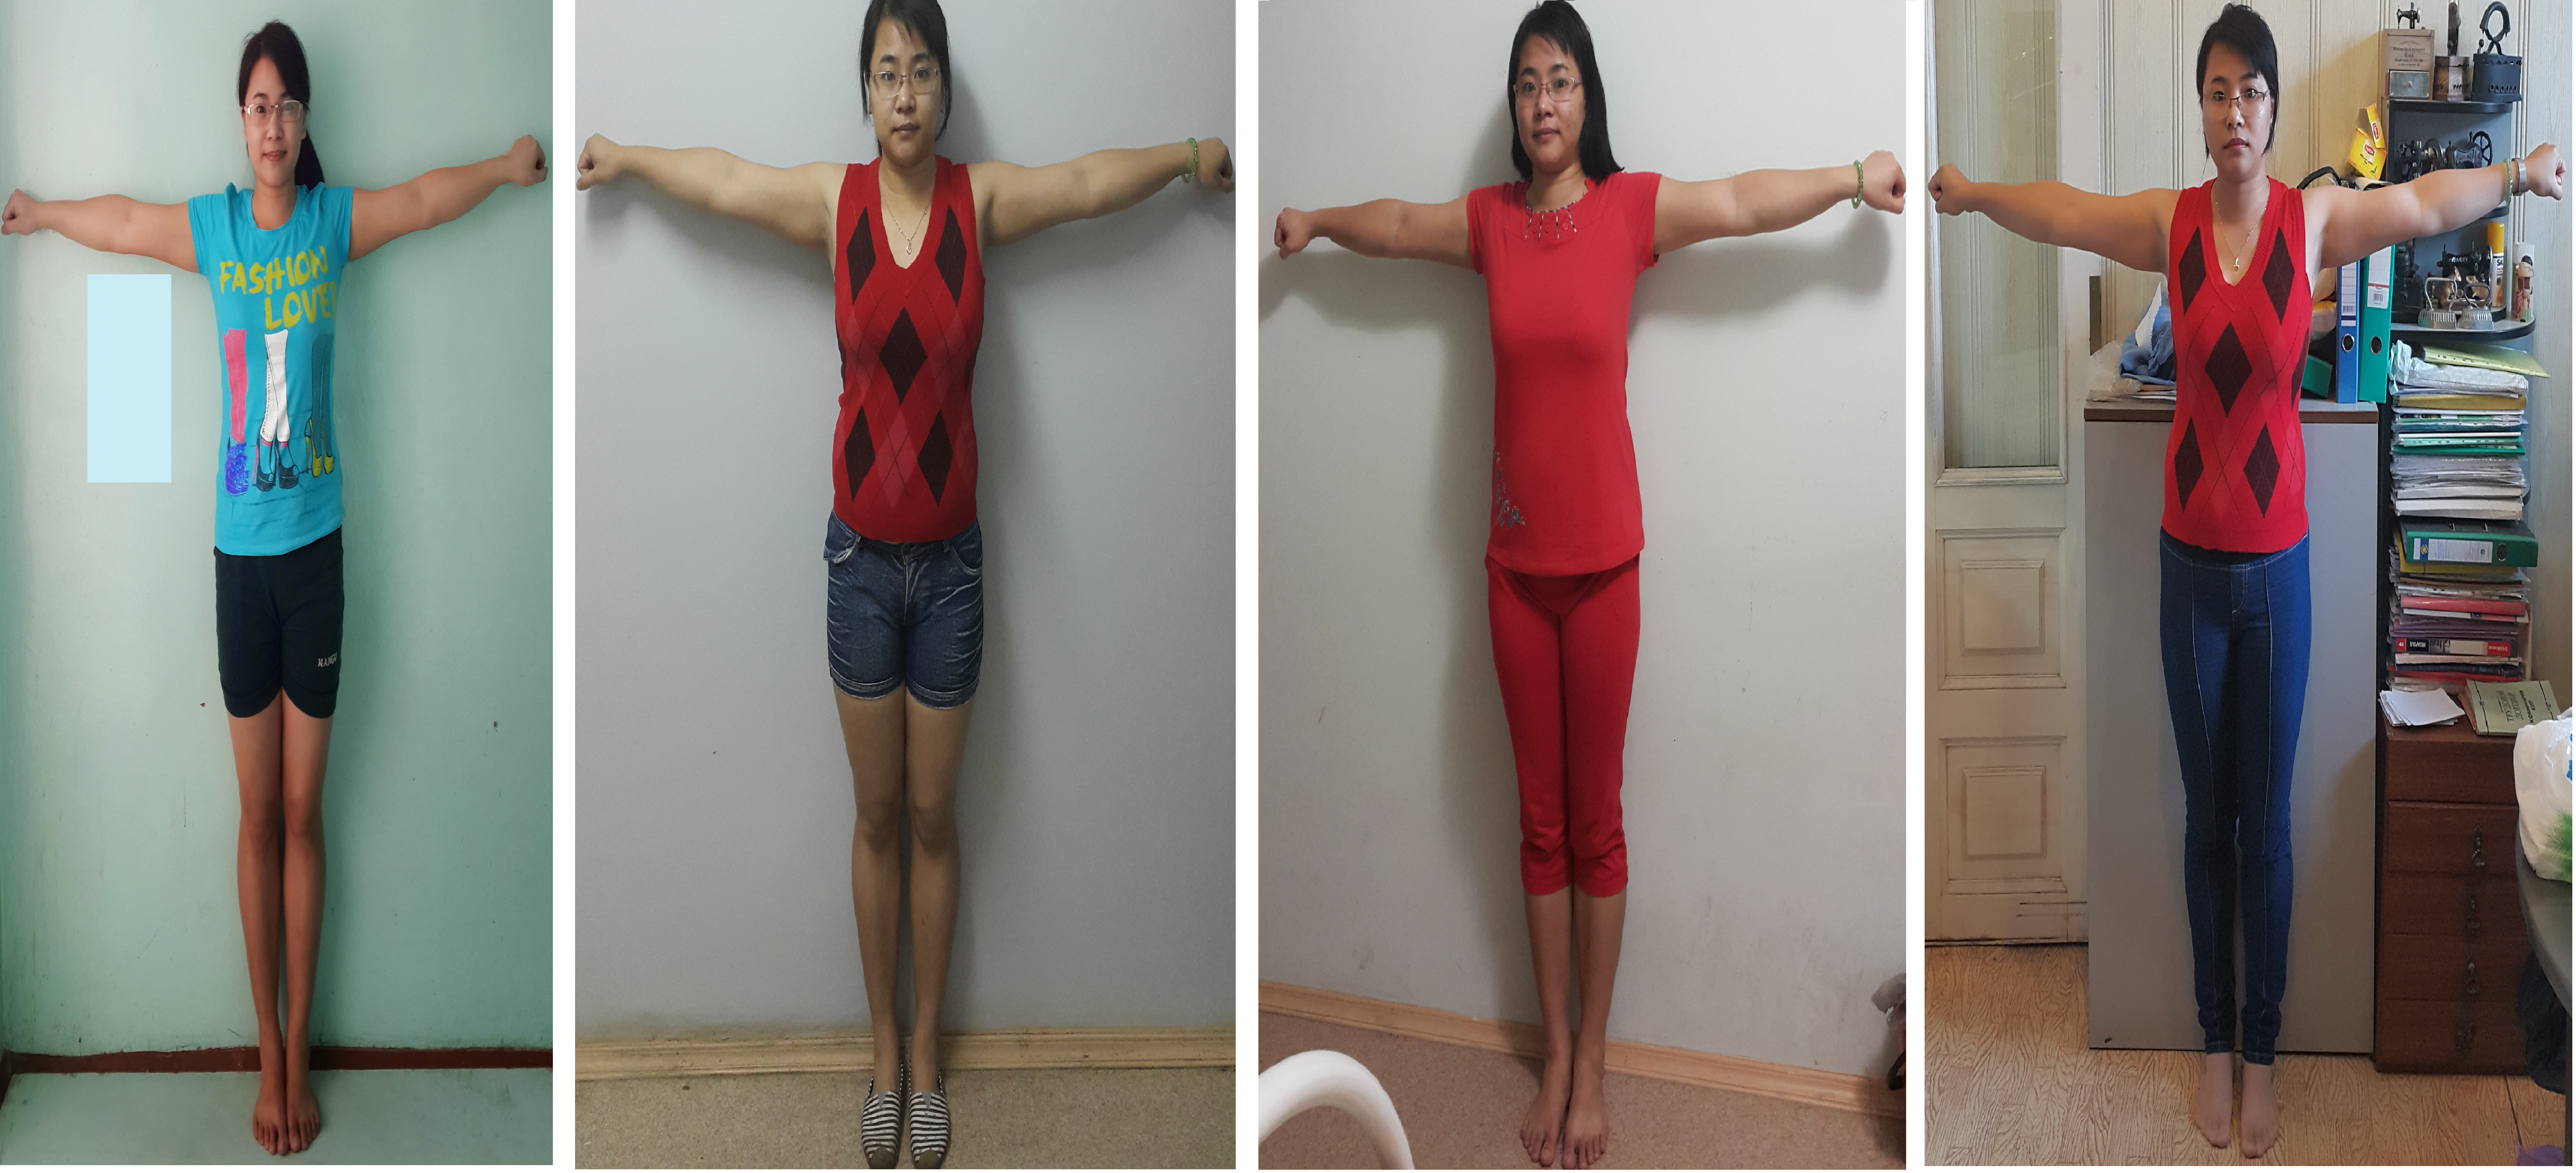
\includegraphics [scale=0.1] {images/h29.png}
\begin{center}
%\captionsetup{justification=justified, labelsep=period}
\caption{Пример данных эксперимента.} \label{img29}
\end{center}
\end{figure}

База данных для экспериментов на компьютере состоит из 6 видео. Эта база данных была создана, чтобы получить данные для тестирования и оценки эффективности работы методов и алгоритмов компьютерного зрения на видео. Создание этой базы необходимо, чтобы учитывать влияние различных факторов на производительность системы (\ref{img36}), (\ref{img37}).

\begin{figure}[ht!]
\centering
\includegraphics [scale=0.5] {images/h36.png}
\begin{center}
%\captionsetup{justification=justified, labelsep=period}
\caption{Результаты извлечения антропометрических признаков и 3D-моделей для женщин.} \label{img36}
\end{center}
\end{figure}
\begin{figure}[ht!]
\centering
\includegraphics [scale=0.5] {images/h37.png}
\begin{center}
%\captionsetup{justification=justified, labelsep=period}
\caption{Результаты извлечения антропометрических признаков и 3D-моделей для мужчин.} \label{img37}
\end{center}
\end{figure}

В ходе эксперимента были использованы алгоритмы компьютерного зрения и извлечения антропометрических признаков. Для этого используются алгоритмы разреза на графах, а также итеративные алгоритмы ближайших точек двух видов: из 24 ключевых точек и 28 ключевых точек для сравнения результата алгоритма вычитания фона и метода выпуклой оболочки \ref{tab7} . В нашей работе \cite{long1} изложен метод измерения различных антропометрических признаков на основе анализа цифровых изображений. Для более эффективного измерения признаков предлагается использовать субпиксельную обработку и анализ выпуклой оболочки. В нашем подходе контур тела описывается выпуклостью дефектов треугольников. Тела представлены треугольниками. Такие треугольники имеют три координаты: выпуклый дефект старт, выпуклый дефект конец, и выпуклый дефект положения точек, соответственно помечены. Мы определили области интересов, которые содержат части тела. Таким образом, мы получили 5 выпуклых областей с соответствующими условиями.

\begin{table}[b!]%
\begin{center}
\caption{Результаты извлечения антропометрических признаков}\label{tab7}
\begin{tabular}{ |c|c|c|c| } 
\hline
  \multirow{3}{*}& Graph-cuts + ICP  & Graph-cuts + ICP  &Вычитание фона \\
								 & (28 ключевых - &(24 ключевых - & + выпуклая\\
	               & - точек)       & - точек)      & оболочка\\
\hline
\multirow{2}{*}{Груди} & \multicolumn{3}{|c|}{93}\\ 
                         & 92.85 & 90.75&85.0 \\ 
\hline
\multirow{2}{*}{Талия} & \multicolumn{3}{|c|}{75}\\ 
                         & 74.80 & 72.0 & 69.79 \\ 	
\hline
\multirow{2}{*}{Бедра} & \multicolumn{3}{|c|}{91}\\ 
                         & 91.3 & 89.65 & 88.65 \\ 
\hline
\multirow{2}{*}{Длина рук} & \multicolumn{3}{|c|}{50}\\ 
                         & 50.40 & 47.62 & 40.30 \\
\hline
\multirow{2}{*}{Обхват } & \multicolumn{3}{|c|}{29}\\ 
                бицепса  & 28.50 & 27.31 & 32.50\\
\hline
\multirow{2}{*}{Обхват } & \multicolumn{3}{|c|}{36}\\ 
                 шеи        & 36.21 & 35.70 & 38.95\\	
\hline
\multirow{2}{*}{Длина } & \multicolumn{3}{|c|}{40}\\ 
                 спины        & 40.10 & 38.75 & 56.50\\	
\hline
\multirow{2}{*}{Ширина } & \multicolumn{3}{|c|}{36}\\ 
                  плеча       & 36.25 & 34.30 & 31.90\\
\hline
\multirow{2}{*}{Длина } & \multicolumn{3}{|c|}{13}\\ 
                 плеча        & 13.10 & 12.83 & 15.56\\
\hline
\end{tabular}
\end{center}
\end{table}%\vspace{10mm}

В (рис. \ref{img24}) описан результат эксперимента проверки точности извлечения антропометрических признаков 3 методов (разреза на графах + ICP для 28 опорных точек, разреза на графах + ICP для 24 опорных точек, вычитание фона + выпуклая оболочка) с ручной метода для одного человека.

\begin{figure}[ht!]
\centering
\includegraphics [scale=0.8] {images/h24.png}
\begin{center}
%\captionsetup{justification=justified, labelsep=period}
\caption{Сравнение результата эксперимента.} \label{img24} \label{img24}
\end{center}
\end{figure}

%-------------------------
\section{Основные результаты и выводы по главе 3}

\begin{enumerate}
	\item В этой главе описывается анализ проектирования систем компьютерного зрения в антропометрии для практических применений: пошив одежды и фитнес-тестирование с помощью аналитических методов объектно-ориентированного UML. Используются диаграммы прецедентов, диаграммы классов и диаграммы последовательности. Классы подробно анализируются, с указанием задач каждой компоненты в программе. Также обоснована целесообразность проектирования приложений компьютерного зрения;
	\item Описаны результаты тестирования алгоритмов компьютерного зрения, в том числе предварительной обработки изображений с помощью фильтра Гаусса, эквализация гистограммы, алгоритм вычитания фона изображения на основе фоновых модели, алгоритм сегментации изображений методом разреза на графах (graph cuts), итеративный алгоритм ближайших точек (Iterative Closest Point - ICP). Алгоритмы функционируют в режиме реального времени и в условиях наличия с шумов в видеопоследовательностях. Эксперименты доказали, что предложенные алгоритмы эффективно работают и включают в себя: извлечение и классификация антропометрических признаков;
	\item Проведен анализ практических результатов экспериментов извлечения антропометрических признаков. Проведено сравнение результатов предложенных методов с методом выпуклой оболочки и вычитания фона по точности. Доказывается преимущество приведенного алгоритма на основе метода разреза графа и итеративного алгоритма ближайших точек;
	\item Результаты экспериментов по классификации антропометрических данных на компьютере и смартфоне показали, что алгоритм случайного леса эффективно работает для решения задач классификации в видеопоследовательностях в режиме реального времени;
	\item Сравнение результатов классификации между алгоритмом случайного леса и алгоритмом Boosting, работающими с видео, показало, что по точности и времени выполнения, более результативный алгоритм случайного леса для системы компьютерного зрения в антропометрии. Алгоритм случайного леса полностью совместим с визуальной системой.
\end{enumerate}

%-------------------------